% Ophaned Sections

\chapter{Orphan Sections}
\label{apx:orphans}
\lhead{Appendix \thechapter. \emph{Orphan Sections}}

\section{Metric Weighting}
\begin{figure}
\begin{subfigure}{.5\textwidth}
  \centering
  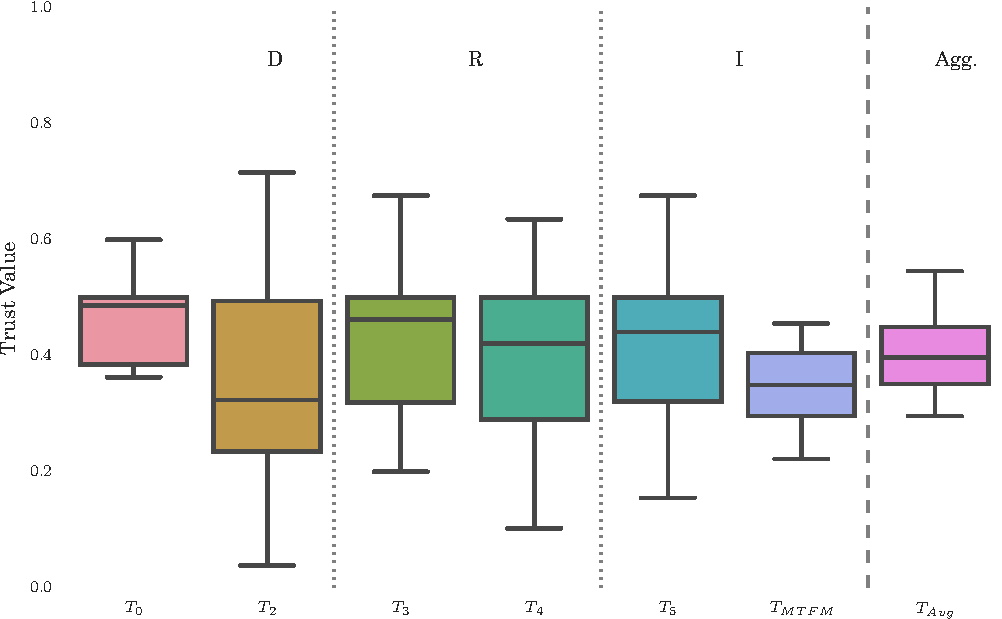
\includegraphics[width=.95\linewidth]{trust_bella_static_selfish}
  %\missingfigure[figwidth=.95\linewidth]{trust bella static selfish}
  \caption{All Nodes Static}
  \label{fig:selfish_trust_static}
\end{subfigure}%
\begin{subfigure}{.5\textwidth}
  \centering
  %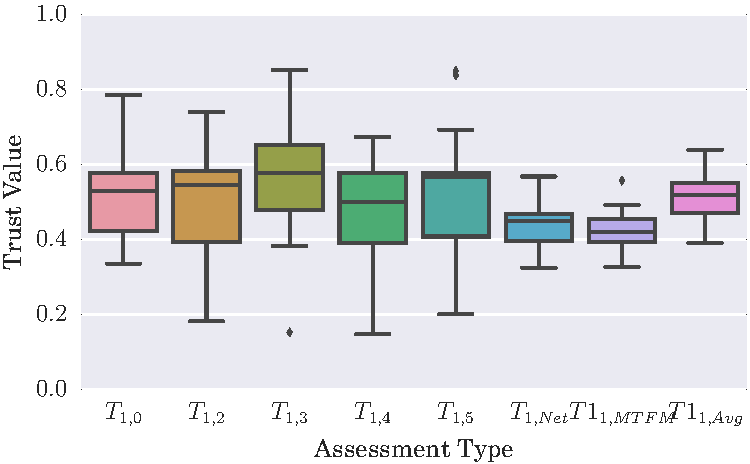
\includegraphics[width=.95\linewidth]{trust_bella_single_mobile_selfish}
  \missingfigure[figwidth=.95\linewidth]{trust bella single mobile selfish}
  \caption{$n_1$ Randomly Walking}
  \label{fig:selfish_trust_single}
\end{subfigure}
\begin{subfigure}{.5\textwidth}
\centering
  %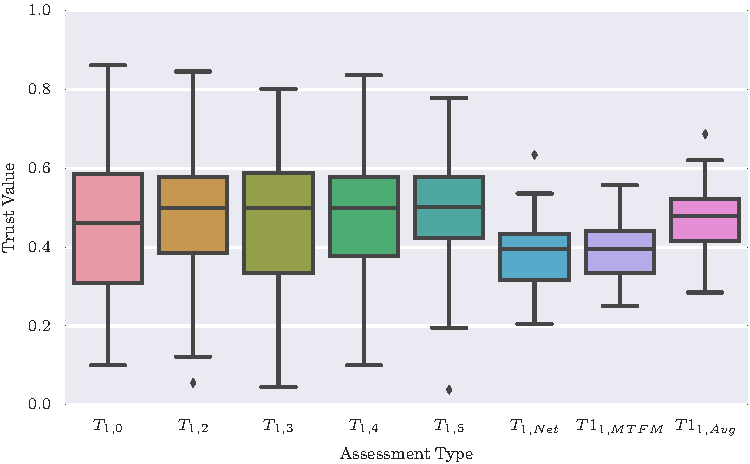
\includegraphics[width=.95\linewidth]{trust_bella_allbut1_mobile_selfish}
  \missingfigure[figwidth=.95\linewidth]{trust bella allbut1 mobile selfish}
  \caption{All Nodes but $n_1$ Randomly Walking}
  \label{fig:selfish_trust_allbut1}
\end{subfigure}
\begin{subfigure}{.5\textwidth}
\centering
  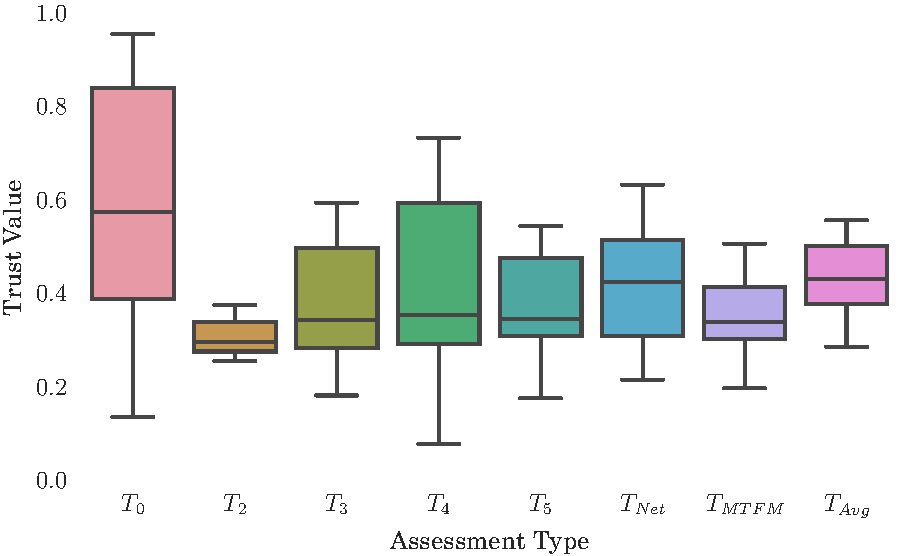
\includegraphics[width=.95\linewidth]{trust_bella_all_mobile_selfish}
  \caption{All Nodes Randomly Walking}
  \label{fig:selfish_trust_all_mobile}
\end{subfigure}
\caption{MTFM Trust assessments for varying mobility options in the selfish case}
\label{fig:trust_mobility}
\end{figure}



\begin{figure}
\begin{subfigure}{0.5\textwidth}
  \centering
  %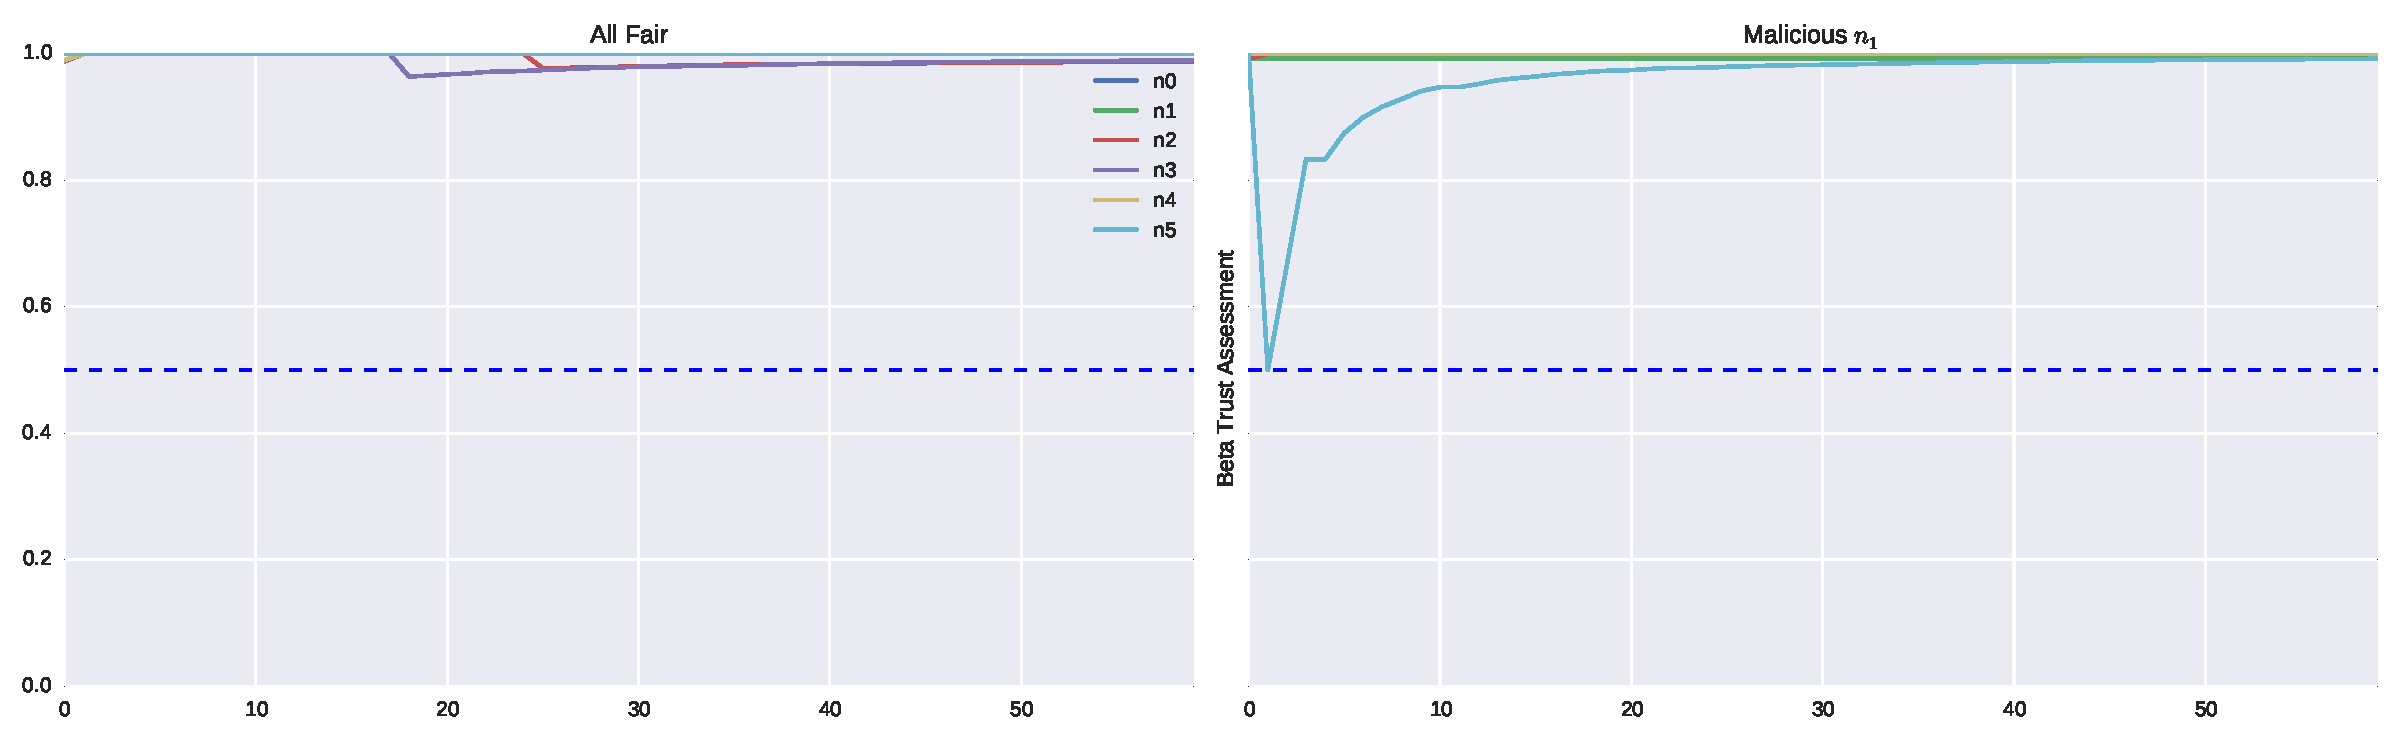
\includegraphics[width=.95\linewidth]{beta_trust_bella_static_joint}
  \missingfigure[figwidth=.95\linewidth]{beta trust bella static joint}
  \caption{All Nodes Static}
  \label{fig:beta_trust_static}
\end{subfigure}%
\begin{subfigure}{0.5\textwidth}
  \centering
  %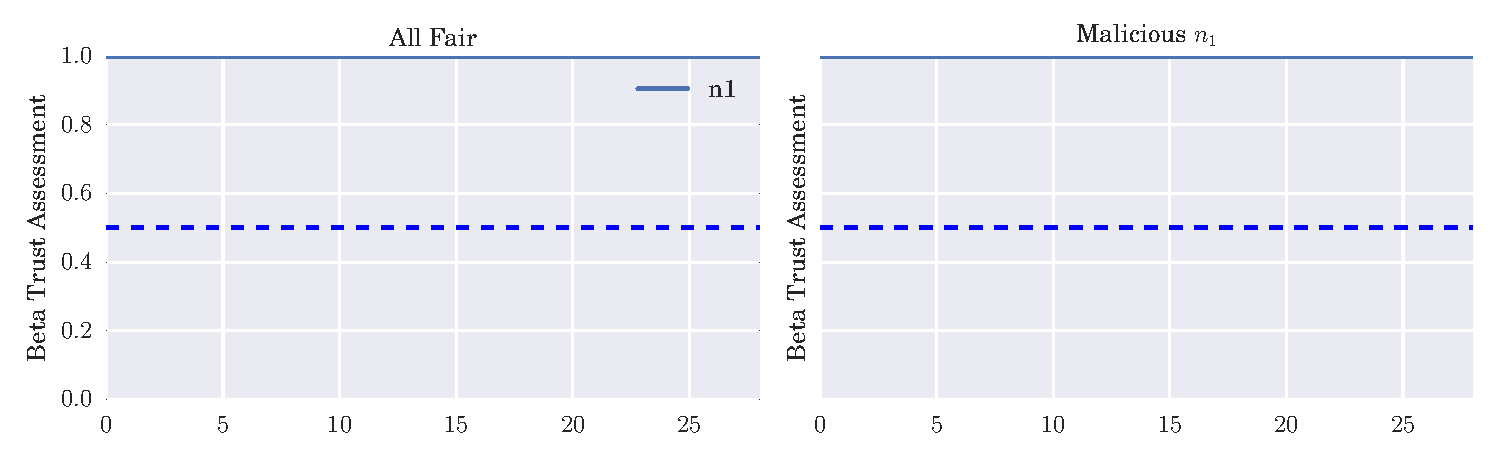
\includegraphics[width=.95\linewidth]{beta_trust_bella_single_mobile_joint}
  \missingfigure[figwidth=.95\linewidth]{beta trust bella single mobile joint}
  \caption{$n_1$ Randomly Walking}
  \label{fig:beta_trust_single}
\end{subfigure}%

\begin{subfigure}{0.5\textwidth}
\centering
  %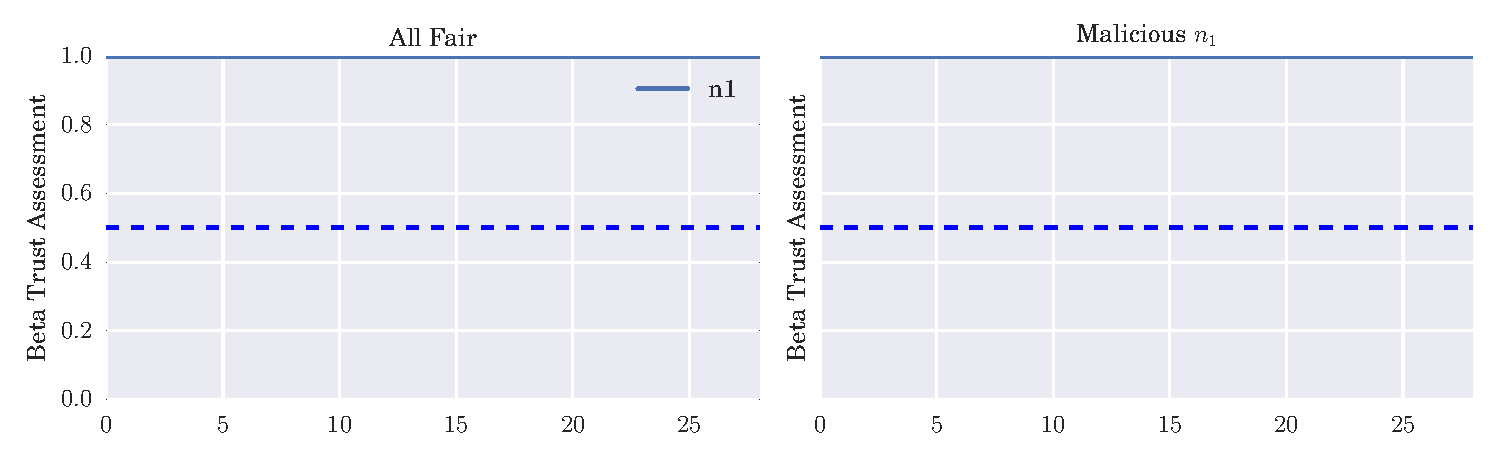
\includegraphics[width=.95\linewidth]{beta_trust_bella_allbut1_mobile_joint}
  \missingfigure[figwidth=.95\linewidth]{beta trust bella allbut1 mobile joint}
  \caption{All Nodes but $n_1$ Randomly Walking}
  \label{fig:beta_trust_allbut1}
\end{subfigure}%
\begin{subfigure}{0.5\textwidth}
\centering
  %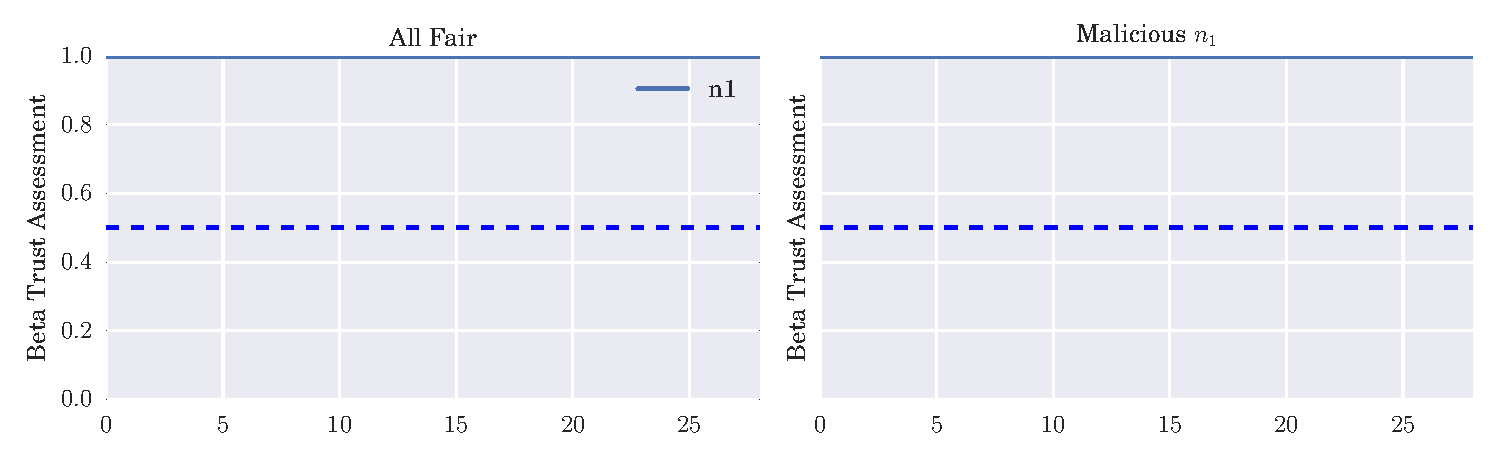
\includegraphics[width=.95\linewidth]{beta_trust_bella_all_mobile_joint}
  \missingfigure[figwidth=.95\linewidth]{beta trust bella all mobile joint}
  \caption{All Nodes Randomly Walking}
  \label{fig:beta_trust_all_mobile}
\end{subfigure}
\caption{Beta Trust time varying assessments for of $n1$ varying mobility options}
\label{fig:trust_mobility}
\end{figure}



\section{UNEDITED PROSE: Real Time Grey Systems}
\emph{Incoming Train of Consciousness}


For a given metric set $X$ such that $X = {x_1,\dots,x_M}$ representing the $M$ different types of measurement generated by an observer. If these metrics are not synchronised, for instance if they are interrupt driven such as communications-based observations, generating more abstract measurements requires inherent assumptions about ``how to accumulate the data while you wait''. For instance, in \cite{Bolster2015}, we demonstrated a periodic trust assessment framework for autonomous marine environments, in such an environment, to establish useful, generalised, data, it was necessary to wait for a relatively long time to accumulate enough data to make assessments.
However, this left many 'smells'; data was being left in-buffer for a long time before being used to make decisions, and by the time the data was collated and processed, it could be wildly different from the reality. Further, while some periods could be extremely sparse or even empty, others could be extremely busy with many records having to be averaged down to provide a 'single period' response. 
Therefore, the implementation of a suitable sequence buffer version of the framework would be beneficial.

Such a sequence buffer framework would involve a tracking predictor that would provide best-guess estimates of an interpolated value for a metric between value updates, and a back-propagation algorithm to retroactively update historical assessments of that metrics so as to better inform any abstracted trust value predictor.

I had initially thought that such a back-propagator would be a total mess as I'd imagined that significant-model-breaking would potentially indicate untrustworthy behaviour, but this is stupid since the per-metric-model has the least information of anyone and is simply there to provide better intermediate values and has no / limited direct impact on the overall trust behaviour. 

This back propagation will probably be a pain to implement as it'd require a retroactive reassessment of trust and could get really messy if it was interrupt driven, but it's better not to prematurely optimise.


\section{From end of Defense Trust Conclusions}
In order to contextualise the discussions on trust in mixed and hybrid networks, an exemplar scenario is considered.
That scenario builds on existing Maritime Autonomy Framework (MAF) investigations(Mollet, J. et al., 2012. Osprey Task 37 Activity 8 - Unmanned Systems Operations: Technical Assurance Work Package - Security Issues and Mitigations - Final Report,)

While the initial assessment does not cover the MHPC PT CONUSE recommendations, it provides a starting point for future trust research in UxV operations.
In order to constrain the scope of this project, a single operational scenario will be analysed within documented MCHP CONUSE(Rudge, A., Chapman, K. \& Goddard, N., 2012. Information Management for MHPC: Research Strategy,), of Route/Area Survey within both peacetime and wartime contexts, with a Beyond Line of Sight (BLOS) operator.
This scenario will be a minimal MCM operation in a littoral area.
In field assets will consist of:
\begin{itemize}
  \item Two squads consisting of Three UUV’s, (tacitly modelled on the in-service REMUS 100 UUV), and a USV providing acoustic-RF relay capabilities per-squad
  \item	an UAV providing BLOS Comms
  \item	A remote human operator (MCMV / PJHQ / etc)
\end{itemize}

\missingfigure{Indicitive Future MCM Scenario}

The differential between the peacetime and wartime contexts will be an attempted capture of a UUV by a manned surface-based FIS asset.
Clearly, this paper has a limited scope and does not attempt to cover every aspect of a trustworthy system.


